\documentclass[10pt,letterpaper,onecolumn,draftclsnofoot]{IEEEtran}
\usepackage[margin=0.75in]{geometry}
\usepackage{listings}
\usepackage{color}
\usepackage{longtable}
\usepackage{graphicx}
\usepackage{float}
\usepackage{tabu}
\definecolor{dkgreen}{rgb}{0,0.6,0}
\definecolor{gray}{rgb}{0.5,0.5,0.5}
\definecolor{mauve}{rgb}{0.58,0,0.82}

\graphicspath{{../images/}}

\lstset{frame=tb,
language=C,
columns=flexible,
numberstyle=\tiny\color{gray},
keywordstyle=\color{blue},
commentstyle=\color{dkgreen},
stringstyle=\color{mauve},
breaklines=true,
breakatwhitespace=true,
tabsize=4
}

\setlength{\parindent}{0cm}

\begin{document}
\begin{titlepage}
	\title{CS 461 - Fall 2016 - Technology Review}
	\author{Matthew Johnson}
	\date{\today}
	\maketitle
	\vspace{4cm}
	\begin{abstract}
		\noindent Abstract goes here
	\end{abstract}

\end{titlepage}

\section{Programming Languages}

At the highest level, a main component of our software defined network
implementation is the programming language it is written in. This is an
important decision to make early in our design, as it affects all choices that
follow.

\subsection{Options}

\subsubsection{Go}

Our first choice is the Go programming language. This is naturally the strongest
choice as the rest of the Ciao infrastructure is written in Go. It would require
a very strong argument to create a separate networking mode in another language.
While technically possible, it would require a great deal of work to make the
different pieces compatible with each other.

\subsubsection{C}

Other than interaction with the rest of the Ciao project, C is another natural
choice. C has been around for decades, and has the capability to do nearly every
computational and networking task. The libraries are extensive and available and
the language is fast.

\subsubsection{Python}

Python is a choice here simply because of its ease of use. Python is very
expressive and has nice libraries that abstract away the complicated details of
software defined networking. The main downfalls of Python, however, are its
reduced speed and space efficiency compared to Go and C. A result of writing a
cloud orchestrator in Python is exemplified in the extremely complicated and
slow Openstack project~\cite{uglyopenstack}.

\subsection{Goals for use in design}

As stated, the choice of programming language will affect all aspects of our
design for this project, from code structure to networking libraries and module
design. This choice will easily have the largest impact on our project.

\subsection{Criteria being evaluated}

Important criteria to consider is the availability of necessary libraries and of
the language and its dependencies itself, the inherent speed of the language to
be used, the security features the language offers, the concurrency
capabilities, and the overall ease of use.

\subsubsection{Availability}

The most available language in terms of libraries and the language itself
(regarding its standard libraries) is obviously C because of how ubiquitous it
is, how universally available it is, and how extensive its standard libraries
are\cite{SOC}.

Close behind C in availability is Python. Python is nearly as available as C is
because of how popular it has become in the last ten years~\cite{PYPL}. Python
has many libraries that provide simple abstractions to networking
functionalities.

Of all these languages, Go is the least available as it is the youngest and
least popular of the three. Go is not normally available by default on most
operating systems and must be installed by the user. Go does, however, have
available libraries that make it very easy to implement networking, as is
evidenced by the extent to which they are used in the Ciao project
currently~\cite{ciao}.

The following figure demonstrates the popularity of C, Go, and Python in the
United States in the last ten years.

\begin{figure}[H]
	\begin{center}
		\makebox[\textwidth]{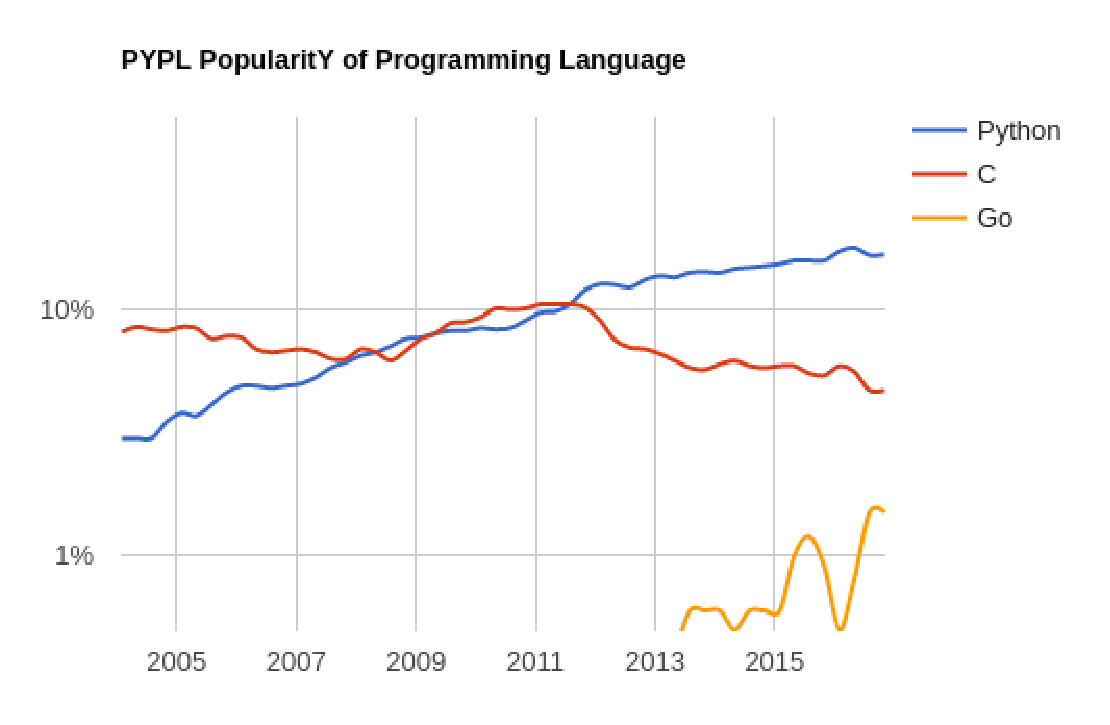
\includegraphics[width=10cm]{pythoncgo.eps}}
		\caption{Python, C, and Go popularity in the US~\cite{PYPL}}
	\end{center}
\end{figure}

\subsubsection{Speed and Space Efficiency}

One benefit of lower-level languages like Go and C is how they treat their
variables. Go and C treat variables differently than some languages such as
Python, which create overhead in order to track type information, and Java,
which converts small ints to Integer class instances when placing them in a
list. An example of this is in the representations of the same value in Go,
Python, and C~\cite{davecheney}:

\begin{lstlisting}
var gocon int32 = 2014              // Go:      4 bytes
uint32_t gocon = 2014;             // C:       4 bytes
gocon = 2014                        #  Python: 24 bytes
\end{lstlisting}

Go performs comparably to C with regard to speed, as well~\cite{benchmarks},
which is considerable since C is often the standard for fast programming
languages. Compared to Python, as would be expected, Go and C can perform up to
45 times faster depending on the workload~\cite{benchmarks}.

\subsubsection{Security}

\subsubsection{Concurrency}

\subsubsection{Ease of use}

\subsection{Direct Comparison}

\begin{center}
	\begin{tabular}{| l | l | l | l | l | l |}
		\hline
		Language & Availability & Efficiency & Security & Concurrency &
		Ease of use \\ \hline
		Go & 3 & 1 & - & - & 1 \\ \hline
		C & 1 & 2 & - & - & 3 \\ \hline
		Python & 2 & 3 & 3 & 3 & 2 \\ \hline
	\end{tabular}
\end{center}

\subsection{Selection}

\section{Networking Libraries}

\subsection{Options}

\subsubsection{}

\subsubsection{}

\subsubsection{}

\subsection{Goals for use in design}

\subsection{Criteria being evaluated}

\subsubsection{Availability}

\subsubsection{Speed}

\subsubsection{Security}

\subsubsection{Concurrency}

\subsection{Discussion}

\subsection{Selection}

\section{Functional Testing Frameworks}

\subsection{Options}

\subsubsection{}

\subsubsection{}

\subsubsection{}

\subsection{Goals for use in design}

\subsection{Criteria being evaluated}

\subsubsection{Availability}

\subsubsection{Speed}

\subsubsection{Security}

\subsubsection{Concurrency}

\subsection{Discussion}

\subsection{Selection}

% Cody
\section{Packet Level Protocols}

\subsection{Options}

\subsubsection{SSNTP}

\subsubsection{}

\subsubsection{}

\subsection{Goals for use in design}

\subsection{Criteria being evaluated}

\subsubsection{Availability}

\subsubsection{Speed}

\subsubsection{Security}

\subsubsection{Concurrency}

\subsection{Discussion}

\subsection{Selection}

%----------------------

\section{nvGRE and VxLAN Switches}

\subsection{Options}

\subsubsection{nvGRE}

\subsubsection{VxLAN}

\subsubsection{}

\subsection{Goals for use in design}

\subsection{Criteria being evaluated}

\subsubsection{Availability}

\subsubsection{Speed}

\subsubsection{Security}

\subsubsection{Concurrency}

\subsection{Discussion}


\subsection{Selection}

%----------------------

\section{GRE/Linux Bridges}

\subsection{Options}

\subsubsection{Linux Bridges}

\subsubsection{}

\subsubsection{}

\subsection{Goals for use in design}

\subsection{Criteria being evaluated}

\subsubsection{Availability}

\subsubsection{Speed}

\subsubsection{Security}

\subsubsection{Concurrency}

\subsection{Discussion}

\subsection{Selection}


%End Cody

\section{References}

\bibliographystyle{IEEEtran}
\bibliography{tech}

\end{document}
